\chapter{Abstraction}

\section{Similarity}

\subsection{Pairing abstractions with similarity measures}

% we have a similarity measure and a way to allow the learner to use it. now ...

Want to remove unimportant structure, while keeping the structure that allows us
to exploit the bellman equation (and thus more efficient search).

Different abstraction spaces support different similarity measures.
State similarity based on value fails in rather simple settings.
But works with state-action abstractions!?

Weaker notions of similarity.
\begin{itemize}
\tightlist
  \item Preserving the ordering of policies. Rather than their absolute value.
  \item Preserving ordering of value. $\phi(s) > \phi(s') \implies Q_{\pi}(s, a) > Q_{\pi}(s', a)$
  \item Preserving the neighbourhoods of policies and their values.
  \item ?
\end{itemize}


\section{LMDPs}

\subsection{LMDP solutions}\label{lmdp-derivation}

% Pick $a \in A$, versus, pick $\Delta(S)$. $f: S\to A$ vs $f:S \to \Delta(S)$.

In the original Todorov paper \cite{Todorov2009}, they derive the LMDP equations for minimising a cost function. This maximisation derivation just changes a few negative signs around.
% Although there is also a subtle change in the interpretation of what the unconstrained dynamics are doing. (??? explain)

\begin{align*}
V(s) &= \mathop{\text{max}}_{u} q(s) - \text{KL}(u(\cdot| s) \parallel p(\cdot | s)) + \gamma \mathop{\mathbb E}_{s' \sim u(\cdot | s)} V(s') \tag{1}\\
\\
&= q(s) + \mathop{\text{max}}_{u} \bigg[ \mathop{\mathbb E}_{s' \sim u(\cdot | s)} \log(\frac{p(s' | s) }{ u(s' | s)}+\gamma \mathop{\mathbb E}_{s' \sim u(\cdot | s)} \big[V(s')\big] \bigg] \tag{2}\\
\log(z_{u^{* }}(s)) &= q(s) + \mathop{\text{max}}_{u} \bigg[ \mathop{\mathbb E}_{s' \sim u(\cdot | s)} \log(\frac{p(s' | s) }{ u(s' | s)}+\mathop{\mathbb E}_{s' \sim u(\cdot | s)} \big[\log(z_{u^{* }}(s')^{\gamma})\big] \bigg] \tag{3}\\
&= q(s) + \mathop{\text{max}}_{u} \bigg[ \mathop{\mathbb E}_{s' \sim u(\cdot | s)} \log(\frac{p(s' | s)z_{u^{* }}(s')^{\gamma} }{ u(s' | s)} ) \bigg] \tag{4}\\
G(s) &= \sum_{s'} p(s' | s) z_{u^{* }}(s')^{\gamma} \tag{5}\\
&= q(s) + \mathop{\text{max}}_{u} \bigg[ \mathop{\mathbb E}_{s' \sim u(\cdot | s)} \log(\frac{p(s' | s)z_{u^{* }}(s')^{\gamma} }{ u(s' | s)} \cdot \frac{G(s)}{G(s)} ) \bigg] \tag{6}\\
&= q(s) + \log G(s) + \mathop{\text{min}}_{u} \bigg[\text{KL}\big(u(\cdot | s) \parallel \frac{p(\cdot | s)\cdot z_{u^{* }}(\cdot)^{\gamma}}{G(s)} \big) \bigg] \tag{7}\\
u^{* }(\cdot | s) &= \frac{p(\cdot | s)\cdot z_{u^{* }}(\cdot)^{\gamma}}{\sum_{s'} p(s' | s) z_{u^{* }}(s')^{\gamma}} \tag{8}\\
\log(z_{u^{* }}(s)) &= q(s) + \log \big(\sum_{s'} p(s' | s) z_{u^{* }}(s')^{\gamma}\big) \tag{9}\\
z_{u^{* }}(s) &= e^{q(s)}\big(\sum_{s'} p(s' | s) z_{u^{* }}(s')^{\gamma}\big) \tag{10}\\
z_{u^{* }} &= e^{q(s)}\cdot P z_{u^{* }}^{\gamma} \tag{11}\\
\end{align*}

By definition, an LMDP is the optimisation problem in (1). We can move the $\text{max}$ in (2), as $q(s)$ is not a function of $u$. Also in (2), expand the second term using the definition of KL divergence, the negative from the KL cancels the second terms negative. (3) Define a new variable, $z(s) = e^{v(s)}$. Also, use the log rule to move the discount rate. (4) Both expectations are under the same distribution, therefore they can be combined. Also, using log rules, combine the log terms. (5) Define a new variable that will be used to normalise $p(s' | s)z(s')^{\gamma}$. (6) Multiply and divide by $G(s)$. This allows us to rewrite the log term as a KL divergence as now we have two distributions, $u(\cdot | s)$ and $\frac{p(\cdot | s)z(\cdot)^{\gamma}}{G(s)}$. (7) The change to a KL term introduces a negative, instead of maximising the negative KL, we minimise the KL. Also in (7) the extra G(s) term can be moved outside of the expectation as it is not dependent in $s'$. (8) Set the optimal policy to minimise the KL distance term. (9) Since we picked the optimal control to be the form in (8), the KL divergence term is zero. (10) Move the log. (11) Rewrite the equations for the tabular setting, where $z$ is vector, and the uncontrolled dynamics are a matrix.

\subsection{MDP Linearisation}\label{mdp-Linearisation}

The ability to solve LMDPs is great, but it's only useful if we can map MDPs into LMDPs, solve them, and map the solution back.
Our goal here is to find a LMDP that has 'similar' structure to the original MDP we were given.\footnotemark[1]

\footnotetext[1]{This derivation is not the same as in Todorov. He sets $b_a \neq r, b_a = r - \sum P \log P$.}

\begin{align*}
\forall s, s' \in S, \forall a \in A, \exists u_a& \;\;\text{such that;} \tag{1}\\
P(s' | s, a) &= u_a(s'|s)p(s'|s) \tag{2}\\
r(s, a) &= q(s) - \text{KL}(P(\cdot | s, a) \parallel u_a(\cdot| s) ) \tag{3}\\
\\
r(s, a) &= q(s) - \text{KL}(P(\cdot | s, a)\parallel\frac{P(\cdot | s, a)}{p(\cdot|s)}) \tag{4}\\
r(s, a) &= q(s) - \sum_{s'}P(s' | s, a) \log(p(s'|s)) \tag{5}\\
\\
m_{s'}[s]&:= \log p(s' | s) \tag{6}\\
D_{as'}[s] &:= p(s'|s, a) \tag{7}\\
c_{s'}[s] &:= q[s] \mathbf 1 - m_{s'}[s] \;\;\text{such that} \;\; \sum_{s'} e^{m_{s'}[s]} = 1 \tag{8}\\
\\
r_a &= D_{as'} ( q \mathbf 1 - m_{s'}) \;\;\forall s \tag{9}\\
r_a &= D_{as'}c_{s'}  \;\;\forall s \tag{10}\\
c_{s'} &= r_aD_{as'}^{\dagger} \;\;\forall s\tag{11}\\
q &= \log \sum_{s'} e^{c_{s'}} \;\;\forall s\tag{12}\\
m_{s'} &= q - c_{s'} \;\;\forall s\tag{13}\\
\end{align*}

We want to pick $p, q$ such that the dynamics of every action in the original MDP can be represented with a control (2),
and every reward generated by an action, can be given by a combination of the
state rewards and the $\text{KL}$-divergence between the true dynamics and a control (3).
Combine (2), (3) to yield (4). Expand the definition of $\text{KL}$-divergence to get (5).
Now, we move to a tabular representation., where $m_{s'}[s]$ and $c_{s'}[s]$ are vectors, and
$D_{as'}[s]$ is a matrix, defined in (6), (7), (8). With these new definitions, we can rewrite equation (5)
as (9). The expectation can be moved to include $q$ because it sums to one.
Substitute equation (8) into (9) to get (10). Solve the linear equation in (11) to get the value of $c_{s'}$.
Use the value of $c_{s'}$ to calculate the state rewards and unconditioned dynamics by using equations (12), (13) and (6).

\section{Symmetries for RL}

\subsection{MDP homomorphisms}\label{mdp-homomorphism}

As pointed out in \ref{C:abstraction}, the notion of an abstraction is captured by a homomorphism.
Given this, it seems natural to extent the defition to MDPs.

A MDP homomorphism is a transformation of a MDP, $\mathcal H: \mathcal M\to \mathcal M$, that preserves the transition and reward function \cite{Ravindran2002}. We can describe this MDP homomorphism as $\mathcal H = (f, g)$ such that;

\begin{align}
P(f(s')|f(s), g_s(a)) = \sum_{s''\in [s']_f} P(s''| a, s) \\
r(f(s), g_s(a)) = r(s, a)
\end{align}

This MDP homomorphism framework yields state-action abstraction, that uses a model based notion of similarity.
However, as pointed out in eariler sections, there are many other possible
notions of abstraction and similarity that can make sense for RL. Specifically, the MDP homomorphism framework
could be generalised in the following ways;

\begin{itemize}
\tightlist
  \item temporal symmetries
  \item approximate symmetries
  \item inference of symmetries under uncertainty
  \item complexity measure / inductive bias
\end{itemize}

% Indeed ...

\subsection{Invariants}

{\color{red}What are the unique differential invariants of $S_2$?!?!}

An important poperty of symmetries is that they can be identified by their generators and relations.

While there are many types of finite group, (cyclic, alternating, ...?) And then there are continuious symmetries, (Lie groups)
Which types of symmetry are important for RL problems?

Let's work through an example, the cart-pole control problem. Your goal is to balance a pole on a cart.
You are allowed to move the cart left or right.

% How hard is it to find these symmetries?
% Are some harder than others?

\begin{figure}[h!]
	\centering
	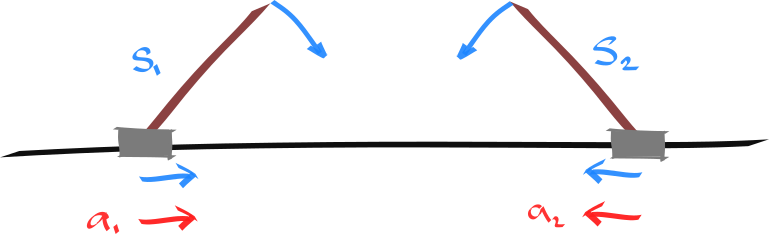
\includegraphics[width=1\textwidth,height=0.25\textheight]{../../pictures/drawings/cart-pole-mirror.png}
	\caption{Two mirror symmetric states of a cart pole. But in what sense are they symmetric?}
\end{figure}

% Need to show this is actually a symmetry, isomorphic to $S_2$?!?
In the case above, the mirrored cart pole is an instance of $S_2$.
The action $f, g$ we apply to the MDP is isomorphism to the simple finite group, $S_2$

Symmetries can be uniquely characterised by their invariants \cite{PeterOlver1999}.
What are the interesting invariants of MDPs? And how do they ???
But, what does this symmetry imply about other quantities of interest for RL?

Invariance, $f(g(x)) = f(x)$, equivariance, $f(g(x)) = g(f(x))$.

In general we want to know;

\begin{itemize}
	\tightlist
	\item We have $n$ different 'symmetries'. But are they really different?
	\item Which symmetries share some invariants?
	\item Which invariants uniquely characterise this symmetry?
\end{itemize}

With this knowledge, we could identify symmetries via their invariants!?!
We can observe invariant properties. (not clear to me how you observe a symmetry!?)

% We briefly explore this in \ref{game-invariants}.

\subsubsection{Cart pole} \label{game-invariants}

\paragraph{Mirror symmetry}

\begin{displayquote}
\textit{What are the invariants of the mirror cart pole example?}
\end{displayquote}

\begin{figure}[h!]
	\centering
	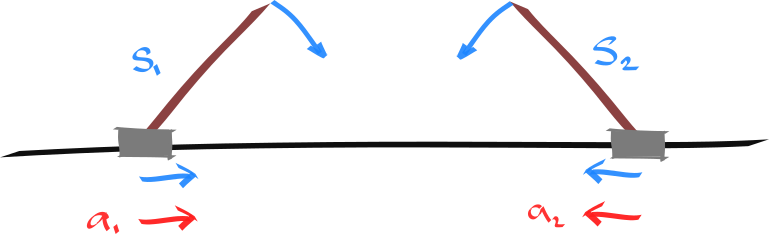
\includegraphics[width=1\textwidth,height=0.25\textheight]{../../pictures/drawings/cart-pole-mirror.png}
	\caption{Two mirror symmetric states of a cart pole.}
\end{figure}

Define the action of $f \in S_2$ on the;

\begin{itemize}
	\tightlist
	\item state space $f \circ s = -s$
	\item action space $f \circ a = -a$
 	\item policy to be $f \circ \pi(a | s) = \pi(f \circ a | f \circ s)$.
	\item transition function to be $(f \circ P)(\cdot | s, a) = P(\cdot| f \circ s, f \circ a)$. ???
\end{itemize}

Therefore, we can write $(f \circ Q^{\pi})(s, a) = Q^{f \circ \pi}(f \circ s, f \circ a)$.
We can write the properties above as;

\begin{align*}
Q^\pi(s, a) &= (f \circ Q^{\pi})(s, a) \tag{expected return}\\
T(Q^\pi)(s,a) - Q^\pi(s,a) &=T(f \circ Q^\pi)(s, a) - (f \circ Q^\pi)(s,a) \tag{Bellman residual}\\
\mathop{\mathbb E}_{s' \sim P(\cdot| s, a)} (s' - s) &= f \circ \mathop{\mathbb E}_{s' \sim (f \circ P)(\cdot| s, a)} (s' - f \circ s) \tag{change in state}\\
\end{align*}
\footnotemark[14]


The rewards (/ value) reachable from $s_1$ are also reachable from $s_2$ (which also implies the converse).
\footnotetext[14]{Note, this assumes we have a 'nice' state representation where differences make sense}

So the expected return, Bellman residual and state transition are invariant to the action of $S_2$.
{\color{red}TODO verify these invariants!?!?}

Is this combination of invariants unique to the mirror symmetry? (how to prove this?!)

\paragraph{Translational symmetry}

\begin{displayquote}
\textit{What are the invariants of the translated cart pole example?}
\end{displayquote}

\begin{figure}[h!]
\centering
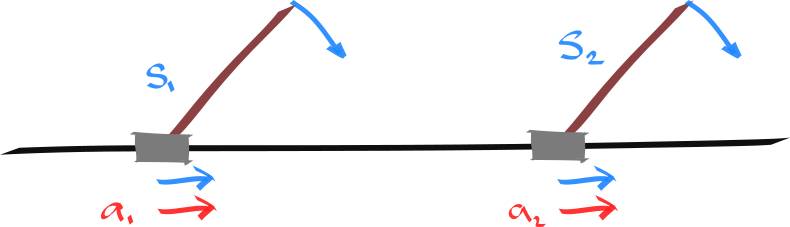
\includegraphics[width=1\textwidth,height=0.25\textheight]{../../pictures/drawings/cart-pole-translation.png}
\caption{Two similar cart poles, which are only a translation different from each other.}
\end{figure}

This is actually a cyclic continuious symmetry, $C_R$.

% How to prove that this is a cts symmetry!?

Define the action of $g \in R$ on the;

\begin{itemize}
	\tightlist
	\item state space $g \circ s = g+s$
	\item action space $g \circ a = a$
 	\item policy to be $g \circ \pi(a | s) = \pi(a | g \circ s)$.
	\item transition function to be $(g \circ P)(s' | s, a) = P(g \circ  s'| g \circ  s,  a)$.
	\item value function to be $(g \circ  Q^{\pi})(s, a) = Q^\pi(g \circ  s,  a)$
\end{itemize}

\begin{align*}
Q^\pi(s, a) &= (g \circ Q^{\pi})(s, a) \tag{expected return}\\
T(Q^\pi)(s,a) - Q^\pi(s,a) &=T(g \circ Q^\pi)(s, a) - (g \circ Q^\pi)(s,a) \tag{Bellman residual}\\
\mathop{\mathbb E}_{s' \sim P(\cdot| s, a)} (s' - s) &= f \circ \mathop{\mathbb E}_{s' \sim (f \circ P)(\cdot| s, a)} (s' - f \circ s) \tag{change in state}\\
\end{align*}

{\color{red}Huh, the key is the action. These have the same invariants!??! No. One is $S_2$, the other is a cts cyclic symmetry...}


\paragraph{Future symmetry}

\begin{figure}[!h]
\centering
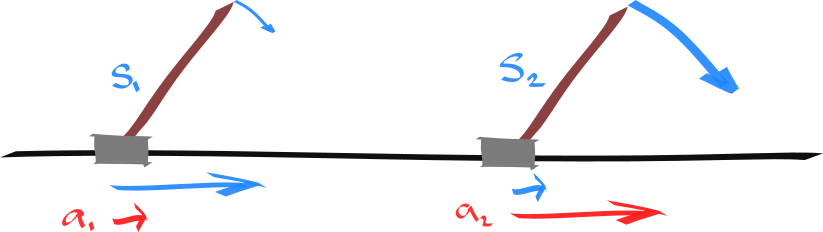
\includegraphics[width=1\textwidth,height=0.25\textheight]{../../pictures/drawings/cart-pole-state.png}
\caption{???}
\end{figure}

Different states, different actions, result in the same next state.
(ahh. $Q$ values are not equivalent if we are have a reward function that punishes larger actions!)


\begin{itemize}
\tightlist
  \item $h \circ (s, a) = ???$
  \item the transition function to be $h\circ P(\cdot|s, a) = P(\cdot|h \circ (s, a))$
  \item the reward function to be $(h \circ r)(s, a) = r(h \circ (s, a))$
  \item the value function to be $(h\circ Q)(s, a) = (h \circ r)(s, a) + \gamma \mathop{\mathbb E}_{s' \sim (h\circ P)(\cdot|s, a)} V(s')$
\end{itemize}

Therefore
\begin{align*}
T(Q)^\pi(s, a) &= T(g \circ Q^{\pi})(s, a) \tag{future expected return}\\
\end{align*}

\paragraph{Temporal symmetry}

{\color{red} this one seems hard. not sure i am going to be able to explicitly construct this one?!}


\begin{figure}[!h]
\centering
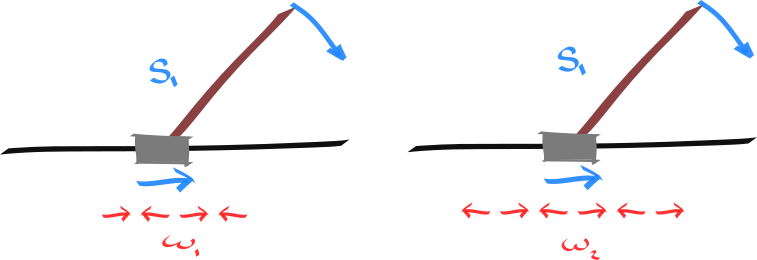
\includegraphics[width=1\textwidth,height=0.25\textheight]{../../pictures/drawings/cart-pole-temporal-approx.png}
\caption{???}
\end{figure}

\begin{align*}
p(\cdot|s_1, \omega_1) = p(\cdot|s_1, \omega_2) \\
Q_{\pi}(s_1, \omega_1) = Q_{\pi}(s_1,\omega_2) \\
\end{align*}


\subsubsection{Pong}

% {\color{red}Need to be more careful with the state / action spaces here. Need to define properly!?}
State = $[p_1, v_1, p_2, v_2, p^x_b, p^y_b, v^x_b, v^y_b]$
Where all of these are centered around the middle.
Action = $\{+x, -x, 0\}$

\paragraph{Mirror symmetry (vertical)}

\begin{figure}[!h]
\centering
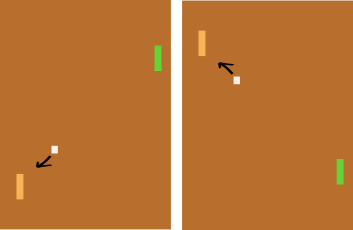
\includegraphics[width=1\textwidth,height=0.25\textheight]{../../pictures/drawings/pong-vert-flip.png}
\caption{???}
\end{figure}


Define the action of $f \in S_2$ on the;

\begin{itemize}
	\tightlist
	\item state space $f \circ [p_1, v_1, p_2, v_2, p^x_b, p^y_b, v^x_b, v^y_b] := [-p_1, -v_1, -p_2, -v_2, -p^x_b, p^y_b, -v^x_b, v^y_b]$
	\item action space $f \circ a := -a$
 	\item policy to be $f \circ \pi(a | s) = \pi(f \circ a | f \circ s)$.
	\item transition function to be $(f \circ P)(s' | s, a) = P(f \circ s'| f \circ s, f \circ a)$.
	\item value function is $(f \circ Q^{\pi})(s, a) = Q^{f \circ \pi}(f \circ s, f \circ a)$
\end{itemize}

\begin{align*}
Q^\pi(s, a) &= (g \circ Q^{\pi})(s, a) \tag{expected return}
\end{align*}


\paragraph{Mirror symmetry (player perspective / horizontal)}

\begin{figure}
\centering
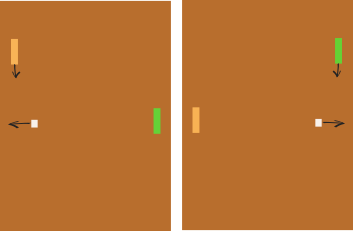
\includegraphics[width=1\textwidth,height=0.25\textheight]{../../pictures/drawings/pong-horz-flip.png}
\caption{???}
\end{figure}

{\color{red}need to fix image. swap colors.}

Define the action of $f \in S_2$ on the {\color{red}(how do we know this is $S_2$)};

\begin{itemize}
	\tightlist
	\item state space $f \circ [p_1, v_1, p_2, v_2, p^x_b, p^y_b, v^x_b, v^y_b] := [-p_1, -v_1, -p_2, -v_2, -p^x_b, p^y_b, -v^x_b, v^y_b]$
	\item action space $f \circ a := -a$
 	\item policy to be $f \circ \pi(a | s) = \pi(f \circ a | f \circ s)$.
	\item transition function to be $(f \circ P)(s' | s, a) = P(f \circ s'| f \circ s, f \circ a)$.
	\item value function is $(f \circ Q^{\pi})(s, a) = Q^{f \circ \pi}(f \circ s, f \circ a)$
\end{itemize}

(\emph{this really requires you to disentangle the model from your
opponent!?})

\begin{align*}
\tau(s'|s, a_{p=0}) &= f_{p=0}(s''|s, a) \cdot f_{p=1}(s'|s'', \hat a) \cdot \pi_{p=1}(\hat a|s'') \\
Q_{p=0}(s, a) &= -Q_{p=1}(s, a)
\end{align*}


\paragraph{Translational symmetry}

\begin{figure}
\centering
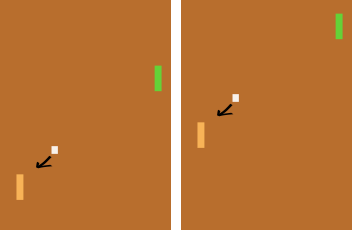
\includegraphics[width=1\textwidth,height=0.25\textheight]{../../pictures/drawings/pong-trans.png}
\caption{???}
\end{figure}

(\emph{although there are boundary cases which cannot be ignored. how
can they be dealt with!?})

\begin{align*}
\forall a: Q_{\pi_1}(s_1, a) = Q_{\pi_2}(s_2, a) \\
\forall a, t: \pi_1(a|s^t_{s^0=s_1}) = \pi_2(a|s^t_{s^0=s_2})
\end{align*}

If we take the same actions, in translated states, we get the same
outcome (up to the boundary conditions).

\paragraph{Temporal symmetries}

\begin{figure}
\centering
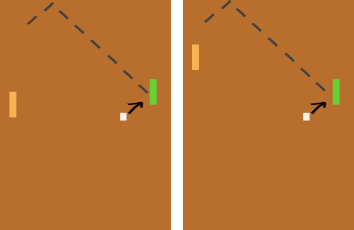
\includegraphics[width=1\textwidth,height=0.25\textheight]{../../pictures/drawings/pong-reach.png}
\caption{???}
\end{figure}

\begin{align*}
\exists \pi_1, \pi_2 \;\;\text{s.t.} \;\; Q^{\pi_1}(s_1, a_1) = Q^{\pi_2}(s_2, a_2)
\end{align*}

The same future state can be reached, and thus the same rewards can be
achieved.


\section{Symmetry and machine learning}

\subsection{Exploitation} \label{symmetric-exploitation}

\begin{displayquote}
\textsl{Once have discovered a symmetry, how might we exploit that knowledge?}
\end{displayquote}

Similar to how we considered how to exploit an abstraction in section \ref{},
let's review some existing methods for exploiting the knowledge of a symmetry. \footnotemark[22]

\footnotetext[22]{Note that, in all of these methods, symmetry provides
advantage over considering just the pairwise similarities. We will return to this later.}

% note: what has been given to these methods of exploitation?
% knowledge of the group, or its actions, or ...?

\paragraph{Exploiting symmetry for efficient control}

If we have a MDP, $M_1$, then solving it via value iteration requires $\mathcal O(\epsilon |S|^2|A|)$ iterations.
However, if we know that there exists symmetries in the state space, then we can 'minimise the model',
by applying the MDP homomorphism $\mathcal H: \mathcal M\to \mathcal M$.
This new, minimised, MDP, $M_2$ has a smaller state space, as $|S_{M_2}| = \frac{|S_{M_1}|}{k}$
and essentially the same dynamics and rewards. Thus we can solve $M_2$, with cost $\mathcal O(\epsilon \frac{|S|^2|A|}{k^2})$
and then lift the solution back to $M_1$. \cite{Dean1997, NARAYANAMURTHY}


\paragraph{Exploiting symmetry for efficient inference}\label{symmetry-inference}

There has been a large amount of work (that we are familiar with) exploring
the exploitation of ... See  here for an overview \ref{symmetry-inference}.

The general essence of the idea is \textit{"invariance reduces variance"}. \cite{Chen2019}

Locomotion sharing ... \cite{Abdolhosseini}

By sharing weights according to group structure\cite{Ravanbakhsh2017a}, we can increase the effective data seen by each weight.

\paragraph{Output coupling}

Mahajan et al. propose to use knowledge similarity to share couple outputs.
\cite{Mahajan2017}

\begin{align*}
\chi: (S\times A) \times (S\times A) \to [0, 1] \\
\mathcal L(\theta) = \mathop{\mathbb E}_{\chi} \Big[(Q(s, a, \theta)-Q(s', a', \theta))^2 \Big]
\end{align*}

Coupling the outputs of similar state-actions. This is nice because, we might know
that $s, a$ and $s', a'$ are similar. Yet we many not have observed $s', a'$.

% Equivalent to sharing training data?!?

However, how did we know that $s, a$ and $s', a'$ are similar without seeing $s', a'$?

- Data sharing (aka duplicate tuples \cite{Ho2019a})

\paragraph{Gradient coupling}

\begin{align*}
\nabla_{\theta} \ell(s, a, \theta) = \nabla_{\theta} \ell(s', a', \theta) \\
\chi \cdot \nabla_{\theta} \mathcal L(\theta)
\end{align*}

If $\chi$ has the structure $\chi((s, a), (s', a')) = \langle \nabla_{\theta}f(s, a, \theta), \nabla_{\theta} f(s', a', \theta) \rangle$ then will couple gradient in a certain way. NTK.

\cite{Ho2019a}

\paragraph{Data augmentation}

Sharing targets between 'similar' inputs.

\paragraph{Architecture}

Weight sharing?!? Weight coupling!?
\cite{Ravanbakhsh2017a,Abdolhosseini}
\cite{Anselmi2019}

\begin{center}\rule{0.5\linewidth}{\linethickness}\end{center}

\begin{displayquote}
\textit{Which method of incorporating knowledge of symmetries is best?}
\end{displayquote}

\begin{itemize}
\tightlist
  \item Data augmentation: flips.
  \item Gradient coupling: ??? gets complicated?
  \item Output coupling: regulariser on similar outputs.
  \item Architecture: mirror weights.
\end{itemize}

Equivalent?! (in this case, or in general?)
What other ways are there? Want to construct the space of possible ways to incorporate symmetries into a learner.


\paragraph{Exploiting symmetry for efficient exploration}

Holtzen et al. \cite{Holtzen2019} show that by grouping together variables according to
the knowledge of a symmetry, they show that \textit{orbit-jump MCMC mixes rapidly in the number of orbits}.
In other words, symmetries allow the efficient estimation of distributions.
% Want to demonstrate this.
% {\color{red}TODO max ent + abstraction experiments}

Also. \cite{Campbell2019}

\begin{center}\rule{0.5\linewidth}{\linethickness}\end{center}

All of these methods rely on a similar type of argument. Picking a representative
of a partition and only using that one. Averaging over orbits. ...


\subsection{Discovery}

Also.

Existing methods of discovery!?!?
 How can it be discovered?

 A couple parts. Discovery of symmetries, exploration of the knowledge of symmetries.

 Unsupervised discovery. Not much success yet. Only when using some kind of supervised signal.

 \cite{Ho2019a, Lim2019, Cubuk2018, Cubuk2019}
 Discover which symmetries apply to a given domain, and at what magnitude.
 The optimisation problem becomes one of picking the probability of each op and its magnitude.
 There is a small set of ops (aka symmetries) that are given:
 \textit{Identity, AutoContrast, Equalize, Rotate, Solarize, Color, Posterize, Contrast,
 	Brightness, Sharpness, ShearX, ShearY, TranslateX, TranslateY.}
 Uses validation error as a reward for learning.


\subsection{Symmetry Examples}

$S_4$

 \begin{align*}
  \begin{bmatrix}
    0 & 1 & 2 & 3 \\
    3 & 0 & 1 & 2 \\
    2 & 3 & 0 & 1 \\
    1 & 2 & 3 & 0 \\
  \end{bmatrix}
  \begin{bmatrix}
    a & b & c & d \\
    d & a & b & c \\
    c & d & a & b \\
    b & c & d & a \\
  \end{bmatrix}
 \end{align*}

$S_2 \times S_2$

 \begin{align*}
  \begin{bmatrix}
    (0, 0) & (0, 1) & (1, 0) & (1, 1) \\
    (0, 1) & (0, 0) & (1, 1) & (1, 0) \\
    (1, 0) & (1, 1) & (0, 0) & (0, 1) \\
    (1, 1) & (1, 0) & (0, 1) & (0, 0) \\
  \end{bmatrix}
 \begin{bmatrix}
   a & b & c & d \\
   b & a & d & c \\
   c & d & a & b \\
   b & c & b & a \\
 \end{bmatrix}
 \end{align*}

 % http://mathworld.wolfram.com/FiniteGroup.html

How many observations are sufficient to discriminate between $S_4$ and $S_2\times S_2$?
What about symmetries of different order?

\subsubsection{Actions}

Let $S_2$ be the group $\big(\{e, g\}, \circ \big)$. Where we represent the action of $e, g$ on the real vectors, $x\in R^n$
as permutation matrices, and the composition operator $\circ$ becomes matrix multiplication, $\cdot$. Therefore $e = I_n$ and $g$ can be one of many possible actions. For example, consider the nine \footnotemark[34] representations of $g$ when applied $R^4$.

\footnotetext[34]{There are no others. Proof by construction. Enumerate all permutations and check which ones are idempotent.}

\begin{align*}
 \begin{bmatrix}
 1 & 0 & 0 & 0 \\
 0 & 1 & 0 & 0 \\
 0 & 0 & 0 & 1 \\
 0 & 0 & 1 & 0 \\
 \end{bmatrix}
 &\begin{bmatrix}
 1 & 0 & 0 & 0 \\
 0 & 0 & 1 & 0 \\
 0 & 1 & 0 & 0 \\
 0 & 0 & 0 & 1 \\
 \end{bmatrix}
 \begin{bmatrix}
 1 & 0 & 0 & 0 \\
 0 & 0 & 0 & 1 \\
 0 & 0 & 1 & 0 \\
 0 & 1 & 0 & 0 \\
 \end{bmatrix}   \\
 \begin{bmatrix}
 0 & 1 & 0 & 0 \\
 1 & 0 & 0 & 0 \\
 0 & 0 & 1 & 0 \\
 0 & 0 & 0 & 1 \\
 \end{bmatrix}
 &\begin{bmatrix}
 0 & 0 & 1 & 0 \\
 0 & 1 & 0 & 0 \\
 1 & 0 & 0 & 0 \\
 0 & 0 & 0 & 1 \\
 \end{bmatrix}
 \begin{bmatrix}
 0 & 0 & 0 & 1 \\
 0 & 1 & 0 & 0 \\
 0 & 0 & 1 & 0 \\
 1 & 0 & 0 & 0 \\
 \end{bmatrix}   \\
 \begin{bmatrix}
 0 & 1 & 0 & 0 \\
 1 & 0 & 0 & 0 \\
 0 & 0 & 0 & 1 \\
 0 & 0 & 1 & 0 \\
 \end{bmatrix}
 &\begin{bmatrix}
 0 & 0 & 1 & 0 \\
 0 & 0 & 0 & 1 \\
 1 & 0 & 0 & 0 \\
 0 & 1 & 0 & 0 \\
 \end{bmatrix}
 \begin{bmatrix}
 0 & 0 & 0 & 1 \\
 0 & 0 & 1 & 0 \\
 0 & 1 & 0 & 0 \\
 1 & 0 & 0 & 0 \\
 \end{bmatrix}   \\
\end{align*}

Each of these actions has the $S_2$ group structure.
But which of these actions are preferable?

Observe that the first two row contain permutations that swaps (two) elements of the vector ($a\leftrightarrow b$).
While the last row of permutations contain permutations that swaps pairs ($(a, b) \leftrightarrow (c, b)$).


\subsubsection{Race grid world}\label{race-grid-world}

% describe the setting. its symmetric bc.
% it makes sense bc...
The type of abstraction used is state abstraction. So we should see BATS scale better with MDPs of increasing state space.

\begin{figure}[h!]
  \centering
  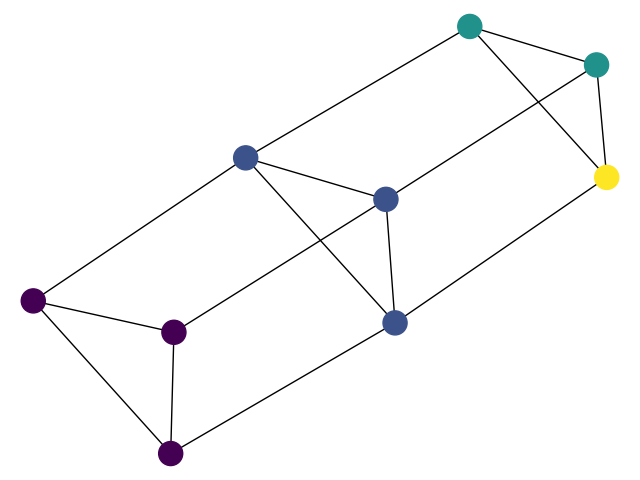
\includegraphics[width=0.7\textwidth,height=0.35\textheight]{../../pictures/figures/race-mdp-puzzle-n3.png}
  \caption{The purple nodes represent the starting states. The green-teal nodes represent states wth reward $1$. There are 5 actions, left, right, up, down, none.
	Starting from the leftmost purple node: Left moves clockwise to the next purple node. Up moves to the blue node. Down doesn't result in movement. None doesn't result in movement.}
\end{figure}



\subsection{n-dimensional Cart pole}\label{action-space-experiments}

\begin{displayquote}
  \textit{How can we test a learners ability to detect symmetries and exploit them?}
\end{displayquote}

We propose a simple test, the n-dimensional cart pole: a generalisation of the
cart pole problem to $n$ dimensions. Rather than receiving observations in
$\mathbb{R}^4$ (the position, velocity, angle and angular velocity), observations are
in $\mathbb{R}^{4\times n}$. And the action space is generalised from $\{0,1\}$ (left and right),
to $\{0,1\}^{n}$.

% What makes this problem hard??
% This setting allows us to easily control the amount of symmetry.
% Existing envs dont test this because!?!?

\subsubsection{How is this problem symmetric?}

The $n$-dimensional cart pole problem can be reduced to $n$, one dimensional cart pole problems.
Where each of these one dimensional cart pole problems cart pole problems is easy to solve.

In a more formal sense. This problem is symmetric because the optimal policy and its ($Q$) values are invariant to the actions of the permutation group of order n, $S_n$.

\begin{align*}
g \circ s_j &= g \circ [x_0, \dots, x_i, \dots, x_{n-1}] \\
&= [x_1, x_0, \dots, x_i, \dots, x_{n-1}] \\
g_i \circ a_k &= g \circ [u_0, \dots, u_i, \dots, u_{n-1}] \\
&= [u_1, u_0 \dots, u_i, \dots, u_{n-1}] \\
g\circ \tau(s'|s, a) &= \tau(g\circ s'|g\circ s, g\circ a) \\
g\circ R(s, a) &= R(g\circ s, g\circ a) \\
g\circ \pi^{* }(a|s) &= \pi^{* }(g\circ a| g\circ s) \\
&= \pi^{* }(a|s) \tag{invariance of the optimal policy}\\
g\circ Q^{\pi^{* }}(s, a) &= Q^{\pi^{* }}(g\circ s, g\circ a) \\
&= Q^{\pi^{* }}(s, a) \tag{invariance of the optimal values}
\end{align*}

{\color{red}do I need to prove this?! via the transition fn / reward fn...}

We describe a state as $s_j = [x_0, \dots, x_i, \dots, x_{n-1}]$, where $x_i = (p_c^i, v_c^i, p_p^i, v_p^i)$. Where, $p_c$ is the position of the cart, $v_c$ is the velocity of the cart, $p_p$ is the position of the pole, $v_p$ is the angular velocity of the pole. We describe actions as $a_k \in \{0, 1\}^n$. Let $g\in S_n$ be the pairwise permutation, swapping the first two elements $(0\to 1)$.

% However, the learner needs to infer these symmetries, so they can be exploited.

% Well, the original cart pole problem has a few symmetries in it (as explored in \ref{}).
% However, by

\subsubsection{An advantage}

\begin{displayquote}
\textit{What advantage is provided by exploiting symmetries?}
\end{displayquote}

If a learner has inferred that the $n$-dimensional cart pole problem can be decomposed into $n$ identical subproblems,
then that means it is gathering $n$ times the data for the one-dimensional cart pole problem.
So, we should see a factor of $n$ speed up in learning.
This is the same argument made here [quotient groups appendix...].

For a learner that doesn't know of the symmetries. How is this problem hard?
The more dimensions there are, the more ways there are to fail.
Consider how exploration is done. In a single dimension, actions are taken with probability  is
taken with some chance of exploring instead.
% How does PPO / PG do exploration?!?!?
Maybe you correctly balanced the pole in all dimensions except one. To bad, you dont get any reward.

\subsubsection{Experiments}

We use OpenAI's Gym \cite{Brockman2016} and Baselines \cite{baselines} to test this environment.

% What about if we rotate the observations. So the observations are not aligned with the actions?
% Or generalising to n+1? Could start the agent off with n+1 dims. But set them to observe nothing / actions do nothing. Until t > T?

Note: 'Average mean reward' refers to the fact that we have averaged (n=5)
the mean reward (per episode). Also note: This reward is the training performance.

\begin{figure}[h!]
  \centering
  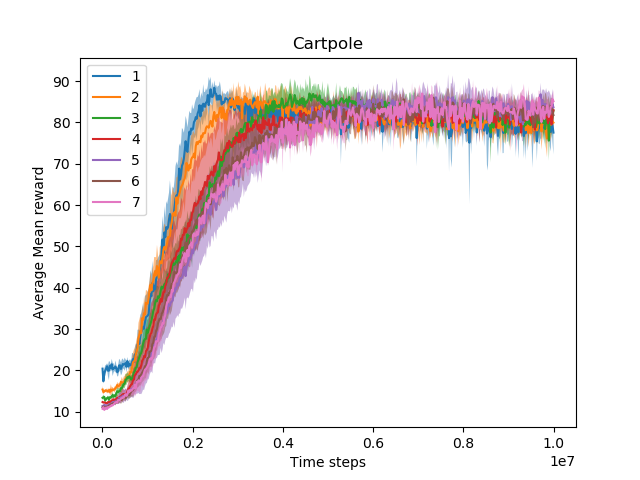
\includegraphics[width=1\textwidth,height=0.5\textheight]{../../pictures/figures/multibinary-nd-cart.png}
  \caption{Default PPO2 solving the nd cartpole problem with access to a \textit{MultiBinary} action space. Each color corresponds to a the average mean return of different, $n$, the number of repeated cart pole problems.}
\end{figure}

As mentioned in the previous section, we expected learning to become much
harder for a learner that doesn't exploit symmetries. These results suggest either of two possibilities:
that PPO2 can discover and exploit symmetries, our setting does not test what we think it does. {\color{red}so... how did we answer this???}

While investigating this further, we realised that the given action space, \textit{MultiBinary}, provies a large amount of information. We ran another test with a \textit{Discrete} action space. Where the learner gets to choose $a\in \mathbb Z_n$.
This action then gets (binary) decoded to the \textit{MultiBinary} format.

A learner that exploits the permutation symmetries in the $n$-dimensional cart pole problem should learn $n$ times quicker.
However, the cost of discovering this permutation symmetry is unknown.

\begin{figure}[h!]
\centering
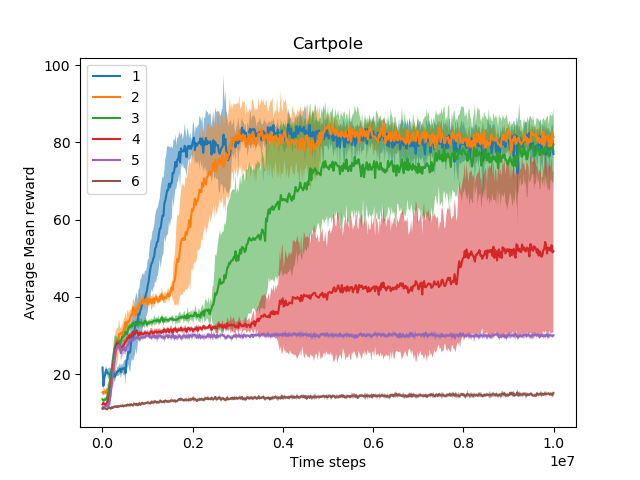
\includegraphics[width=1\textwidth,height=0.5\textheight]{../../pictures/figures/discrete-nd-cart.png}
\caption{Default PPO2 solving the nd cartpole problem with access to a \textit{Discrete} action space. Each color corresponds to a the average mean return of different, $n$, the number of repeated cart pole problems.}
\end{figure}



% It seems surprising that access to the \textit{MultiBinary} action space provides such an advantage.
% Also, it seems surprising that the an increase of 6 dimensions only results in approximately a ~2 million increase in the data required.
% Is the learner doing some sort of intelligent sharing?
% Why is it so hard for the Discrete learner? What operation does it find hard to learn. The ability to decode? $n$ bits to $2^n$ onehots?

% Also, interesting to note that the 1D learner equipped with a \textit{Discrete}
% action space achieves max performance at ~1.75 million samples, while the learner
% equipped with a \textit{MultiBinary} action space achieves max performance at ~2.25 million samples. (significant??)


Future work. The hardness of learning a binary decoder is not sufficient to explain the difference between the
\textit{Discrete} and \textit{MultiBinary} action spaces.
